\documentclass[tikz,border=5pt]{standalone}
\usepackage[T1]{fontenc}
\usepackage{lmodern,amsmath,amssymb}
\usetikzlibrary{arrows.meta,calc,positioning,fit,backgrounds,shapes.geometric,matrix,decorations.pathreplacing,patterns}
\definecolor{ink}{gray}{0.08}
\definecolor{wash}{gray}{0.965}
\definecolor{soft}{gray}{0.45}
\tikzset{box/.style={draw=ink,line width=.65pt,fill=white,align=center,inner sep=4pt,outer sep=0pt,font=\small},flow/.style={draw=ink,line width=.65pt,-{Latex[length=1.8mm,width=1.3mm]},rounded corners=2pt},annotation/.style={font=\scriptsize,text=soft,align=center},groupbox/.style={draw=soft,dashed,line width=.45pt,fill=wash}}
\begin{document}
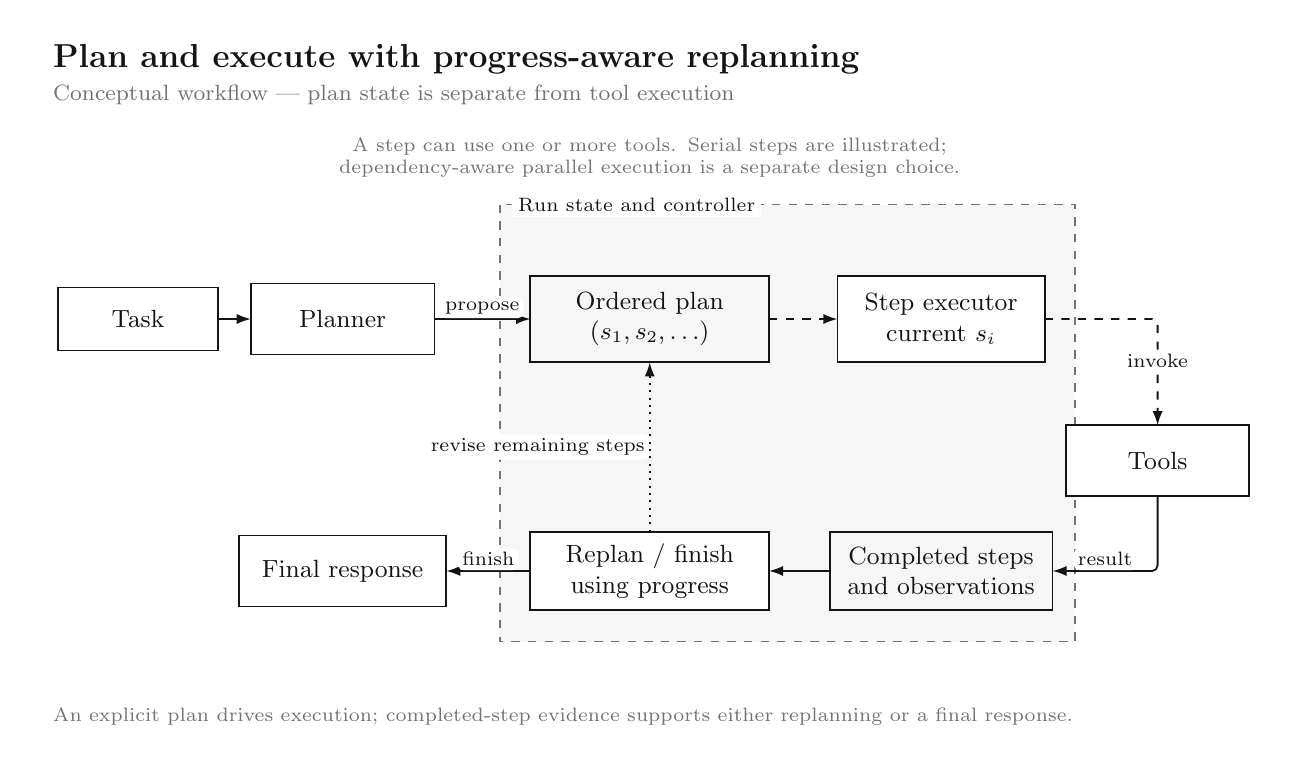
\begin{tikzpicture}[x=1cm,y=-1cm,font=\rmfamily,text=ink]

\path[use as bounding box] (0,0) rectangle (16,9);
\node[anchor=west,font=\large\bfseries] at (.2,.4) {Plan and execute with progress-aware replanning};
\node[anchor=west,font=\footnotesize,text=soft] at (.2,.85) {Conceptual workflow | plan state is separate from tool execution};
\begin{pgfonlayer}{background}
\draw[groupbox] (6.0,2.25) rectangle (13.3,7.8);
\node[anchor=west,font=\scriptsize,fill=white,inner sep=2pt] at (6.15,2.25) {Run state and controller};
\end{pgfonlayer}
\node[box,minimum width=2.0cm,minimum height=0.8cm,text width=1.75cm] (task) at (1.4,3.7) {Task};
\node[box,minimum width=2.3cm,minimum height=0.9cm,text width=2.05cm] (planner) at (4.0,3.7) {Planner};
\node[box,fill=wash,minimum width=3.0cm,minimum height=1.1cm,text width=2.75cm] (plan) at (7.9,3.7) {Ordered plan\\$(s_1,s_2,\ldots)$};
\node[box,minimum width=2.6cm,minimum height=1.1cm,text width=2.35cm] (executor) at (11.6,3.7) {Step executor\\current $s_i$};
\node[box,minimum width=2.3cm,minimum height=0.9cm,text width=2.05cm] (tools) at (14.35,5.5) {Tools};
\node[box,fill=wash,minimum width=2.8cm,minimum height=1.0cm,text width=2.55cm] (record) at (11.6,6.9) {Completed steps\\and observations};
\node[box,minimum width=3.0cm,minimum height=1.0cm,text width=2.75cm] (replan) at (7.9,6.9) {Replan / finish\\using progress};
\node[box,minimum width=2.6cm,minimum height=0.9cm,text width=2.35cm] (response) at (4.0,6.9) {Final response};
\begin{pgfonlayer}{background}
\draw[flow] (task.east) -- (planner.west);
\draw[flow] (planner.east) -- (plan.west) node[midway,above,fill=white,inner sep=1.5pt,font=\scriptsize] {propose};
\draw[flow,dashed] (plan.east) -- (executor.west);
\draw[flow,dashed] (executor.east) -- (14.35,3.7) -- (tools.north) node[midway,above,fill=white,inner sep=1.5pt,font=\scriptsize] {invoke};
\draw[flow] (tools.south) -- (14.35,6.9) -- (record.east) node[midway,above,fill=white,inner sep=1.5pt,font=\scriptsize] {result};
\draw[flow] (record.west) -- (replan.east);
\draw[flow,dotted] (replan.north) -- (plan.south) node[midway,left,fill=white,inner sep=1.5pt,font=\scriptsize] {revise remaining steps};
\draw[flow] (replan.west) -- (response.east) node[midway,above,fill=white,inner sep=1.5pt,font=\scriptsize] {finish};
\end{pgfonlayer}
\node[annotation,anchor=center,text width=13cm] at (7.9,1.65) {A step can use one or more tools. Serial steps are illustrated; dependency-aware parallel execution is a separate design choice.};
\node[anchor=west,align=left,font=\scriptsize,text=soft,text width=15.6cm] at (.2,8.75) {An explicit plan drives execution; completed-step evidence supports either replanning or a final response.};
\end{tikzpicture}
\end{document}
